\documentclass[a4paper,12pt]{article}
\usepackage[english]{babel}
\usepackage[utf8]{inputenc}

%
% For alternative styles, see the biblatex manual:
% http://mirrors.ctan.org/macros/latex/contrib/biblatex/doc/biblatex.pdf
%
% The 'verbose' family of styles produces full citations in footnotes, 
% with and a variety of options for ibidem abbreviations.
%
\usepackage{graphicx}
\usepackage{csquotes}
\usepackage[style=verbose-ibid,backend=bibtex]{biblatex}
\bibliography{sample}

\title{Markovian Approach to Positive-only Problems}

\author{Shayan Amani}

\begin{document}
\maketitle

\section{Preliminaries}

\section{Bounding}
We can use available inequalities to bound our solution. We are always interested in finding upperbound for the policies or solution we propose. Hence, by applying those inequalities -based on requirements of each of them- the upper-bound can be found. Confidence intervals come into the problem where the results are bounded with an upper-bound. Moreover, confidence intervals are authentic measures of reliability of a solution.

    \subsection{Markov's Inequality}
The most simplistic inequality among the other described here in terms of being realxed about the constraints and requirements. The only requirement that needs to be satisfied is $X \geq 0$.
\begin{equation}
\mathrm {P}(X \geq a ) \leq \frac { \mathrm { E}( X ) } { a }
\end{equation}

    \subsection{Chebyshev's Inequality}
    \subsection{Chernoff bound}


\section{Methodology}


\section{Case Study}
The current case is a study on an invasive plant (non-native to the ecosystem) in New England area, namely glossy buckthorn [capitalization?].


% 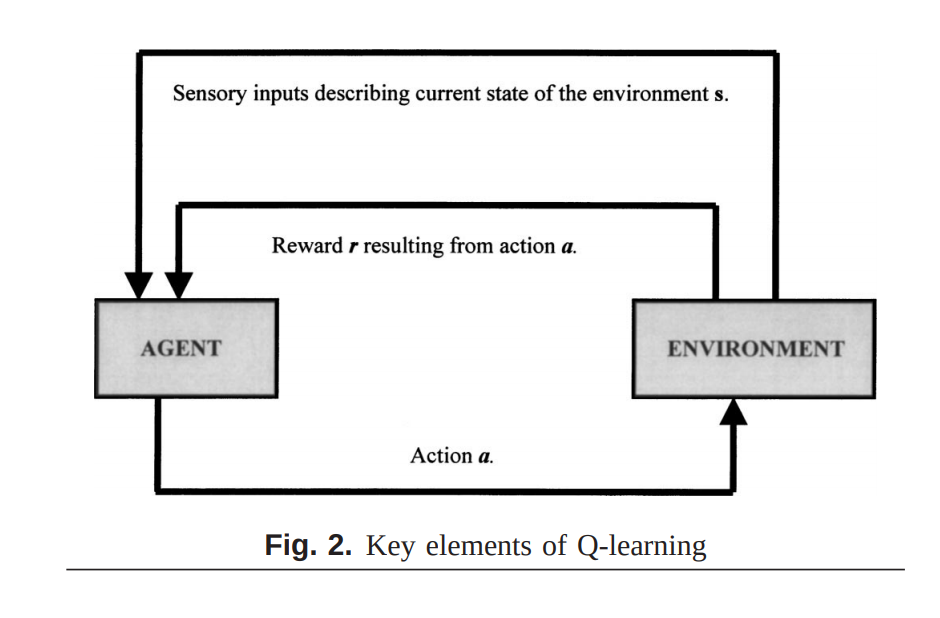
\includegraphics[width=1\columnwidth]{elements.png}



% This is an example citation \autocite{ginsberg}.
% \lipsum[1] % dummy text

% This is another example citation \autocite{brassard}.
% \lipsum[2] % dummy text

% This is a repeated citation \autocite{brassard}.
% \lipsum[3] % dummy text

% This is another example citation \autocite{adorf}.
% \lipsum[4] % dummy text 

\end{document}